\chapter{A Structural Model of Reliability in SoTS}\label{ch:approach}
The systematic literature review presented in \chref{subsec:literature-review-results-reliability} shows that reliability is widely recognized in SoTS research, being discussed in \xofyp{41}{80} studies. However, it is predominantly treated as a reactive architectural concern rather than as a formally modeled system property. Most works emphasize practical mechanisms such as fallback strategies, synchronization, and runtime monitoring \cite{alam2017c2ps, larsen2024towards, acharya2023twins, liu2020web-based, esterle2021digital, villalonga2021decision-making}, while only two studies introduce explicit reliability models and three evaluate reliability through fault injection or simulation \cite{park2020digital, saraeian2022digital}. This imbalance shows that, although reliability is recognized as important, it is not yet systematically integrated into SoTS architectures. This motivates a more structured approach.

\section{Reliability in SoTS}
In dependability theory, reliability is defined as the ability to deliver correct and continuous service \cite{avizienis2001fundamental}. A system is considered unreliable when it ceases to function as intended \cite{randell1978reliability}. To preserve service, fault tolerance mechanisms are introduced to detect, isolate, and recover from faults and errors \cite{hanmer2013patterns}.

Extending this view to SoS, \citet{ferreira2023towards} define reliability as the ability of a SoS to accomplish its mission despite disturbances. These disturbances may arise from interdependencies, constituent evolution, temporary inability to meet demand, or undesired emergent behavior. Interdependencies increase the risk of cascading effects, behavioral changes disrupt coordination, temporary performance issues can impair mission execution even without failure, and emergent behaviours may generate negative global outcomes despite local correctness \cite{ferreira2021reliability}.

To illustrate this, we revisit the illustrative scenario introduced in \chref{ch:example}. Consider a SoTS in which multiple DTs contribute event streams to a CEP engine responsible for monitoring an industrial process. The collective capability of the SoTS, such as detecting abnormal conditions, depends on the correctness and availability of these event streams. During operation, several situations may arise:

\begin{itemize}
    \item A constituent DT temporarily suspends event transmission during peak demand due to maintenance or resource constraints
    \item A constituent DT reduces its event sampling rate due to performance limitations
    \item A constituent DT continues transmitting events while producing incomplete or stale data
\end{itemize}

In isolation, variations in constituent behavior do not necessarily constitute system-level failure. A DT may suspend transmission, reduce event frequency, or operate in a degraded mode according to local constraints while the SoTS remains structurally operational. However, these variations directly constrain the capability of the SoTS and may affect higher-level correlation and inference. Because system-level capability emerges from coordinated interaction among digital services, reliability in SoTS depends not only on local correctness but also on constituent condition and participation dynamics. Disturbance handling cannot be separated from lifecycle, as joining, departure, and behavioral changes reshape dependencies and influence collective stability.

\section{Constituent Lifecycle in SoS}
The most developed lifecycle model of constituent participation in the SoS literature is proposed by \citet{axelsson2019refined} (Figure~\ref{fig:sos-lifecycle-model}). The model defines four structural states: \textit{Ignorant}, \textit{Prepared}, \textit{Passive}, and \textit{Active}. 

\begin{figure}[htp]
\centering
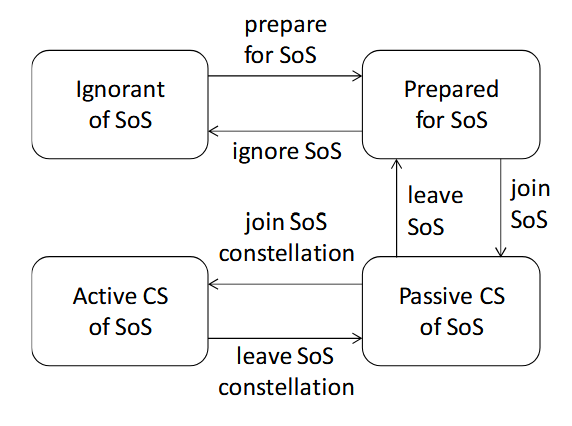
\includegraphics[width=0.5\linewidth]{figures/Approach/SoS Lifecycle Axelsson.png}
\caption{SoS Lifecycle from \citet{axelsson2019refined}}
\label{fig:sos-lifecycle-model}
\end{figure}

An \textit{Ignorant} system possesses relevant capability but does not meet participation requirements. It becomes \textit{Prepared} once technical, organizational, or contractual conditions are satisfied. A \textit{Prepared} system transitions to \textit{Passive} upon formally joining the SoS, and becomes \textit{Active} when it contributes to a specific SoS capability through coordinated interaction with other constituents.

While the lifecycle model of \citet{axelsson2019refined} captures constituent belonging and capability contribution, participation is defined primarily by organizational and contractual readiness. Once requirements are satisfied, participation remains autonomous and independent of constituent condition. Reliability is considered external to lifecycle management. In SoTS environments with tightly coupled digital services, however, unrestricted participation can destabilize capability. DT services dependent on synchronized state and consistent event streams are sensitive to abrupt withdrawal or degraded contribution. Stronger regulation of participation is therefore required to preserve capability under dynamic conditions.

\section{Proposal: Reliability Assessment Levels in SoTS}
Although reliability is widely recognized as essential in SoTS environments (\secref{subsec:literature-review-results-reliability}), constituent lifecycle has been formally modeled \cite{axelsson2019refined}, and SoS reliability has been extensively studied \cite{ferreira2024framework, abdelmoumen2026comprehensive, uday2015designing, ferreira2021reliability, ferreira2023towards}, no framework explicitly links reliability to lifecycle governance. As a result, reliability remains primarily a service-level concern, where recovery mechanisms are applied only after instability manifests.

This work proposes reliability assessment levels defined at the SoTS lifecycle level. The central premise is that reliability can be strengthened not only through fault detection and recovery, but through structured regulation of participation itself. By progressively constraining how constituents join, leave, and reconfigure within the SoTS, architectural intervention is shifted earlier in the disturbance evolution process. This reduces propagation, prevents unsafe integration, and limits the structural conditions under which disturbances arise.

\subsection{Progressive Reliability Levels for SoTS}
\begin{table}[htp]
\centering
\footnotesize
\setlength{\tabcolsep}{5pt}
\begin{tabular}{p{2.2cm} p{4.5cm} p{2cm} p{4cm}}
\toprule
\textbf{Level} & \textbf{Refinement} & \textbf{Intervention Point} & \textbf{Disturbance Coverage} \\
\midrule

L1 -- Reactive 
& Joining, departure, and role changes must be announced. Participation remains uncontrolled but becomes structurally visible. 
& During/after impact 
& Improves detection of interdependency cascades \newline 
limited influence on evolution or temporary inability \\

L2 -- Proactive 
& Joining and departure are delayed through enforced notice periods, buffering structural change and reducing instability. 
& Before impact 
& Mitigates disruption from constituent evolution and temporary inability \newline
reduces cascade severity \\

L3 -- Controlled 
& Participation becomes conditional, with enforceable obligations, admission approval, and regulated withdrawal. 
& Before formation 
& Prevents unstable integration and abrupt withdrawal \newline
strongly addresses evolution-driven disturbances \\

L4 -- Adaptive 
& Responsibilities may be reassigned to preserve capability, enabling structural reconfiguration under change. 
& Before structural conditions 
& Actively compensates for structural loss \newline
mitigates interdependencies, evolution, and partial capability degradation \\

\bottomrule
\end{tabular}
\caption{Reliability Levels}
\end{table}
\citet{axelsson2019refined}'s lifecycle model characterizes constituent participation but leaves the precise semantics of transitions application-specific. The proposed work preserves \citet{axelsson2019refined}'s original lifecycle states and transition semantics while extending the model through additional refinements. Minor terminological adjustments are introduced---\textit{Ignorant} is renamed to \textit{Disengaged}, and \textit{Ignore SoS} to \textit{Disengage from SoTS}---but all original states and transitions retain their intended meaning.

Inspired by staged maturity frameworks \cite{paulk1993capability}, we define four progressive reliability levels that refine and extend the lifecycle by introducing increasing architectural regulation of constituent participation behaviour. Across the presented state charts, higher reliability levels shift the point of intervention earlier in the disturbance progression \cite{ferreira2023towards}. Rather than relying solely on reactive service-level compensation after structural change, the refined lifecycle progressively enables preventive and adaptive structural regulation of participation itself.

\subsubsection{Level 1: Reactive}
\citet{axelsson2019refined} notes that when joining, other constituent systems must become aware of the new participant to address it and establish necessary security precautions. Level 1 formalizes this requirement by encoding explicit announcement actions into the state chart. Transitions into and out now require announcement before completion, introducing visibility without restricting participation.

With respect to disturbances, this level primarily mitigates risks arising from interdependencies. By making participation changes observable, cascading effects caused by unexpected structural modifications can be detected earlier. However, intervention still occurs at or immediately after disturbance impact, and service-level compensation remains the primary recovery mechanism.


\begin{figure}[htp]
\centering
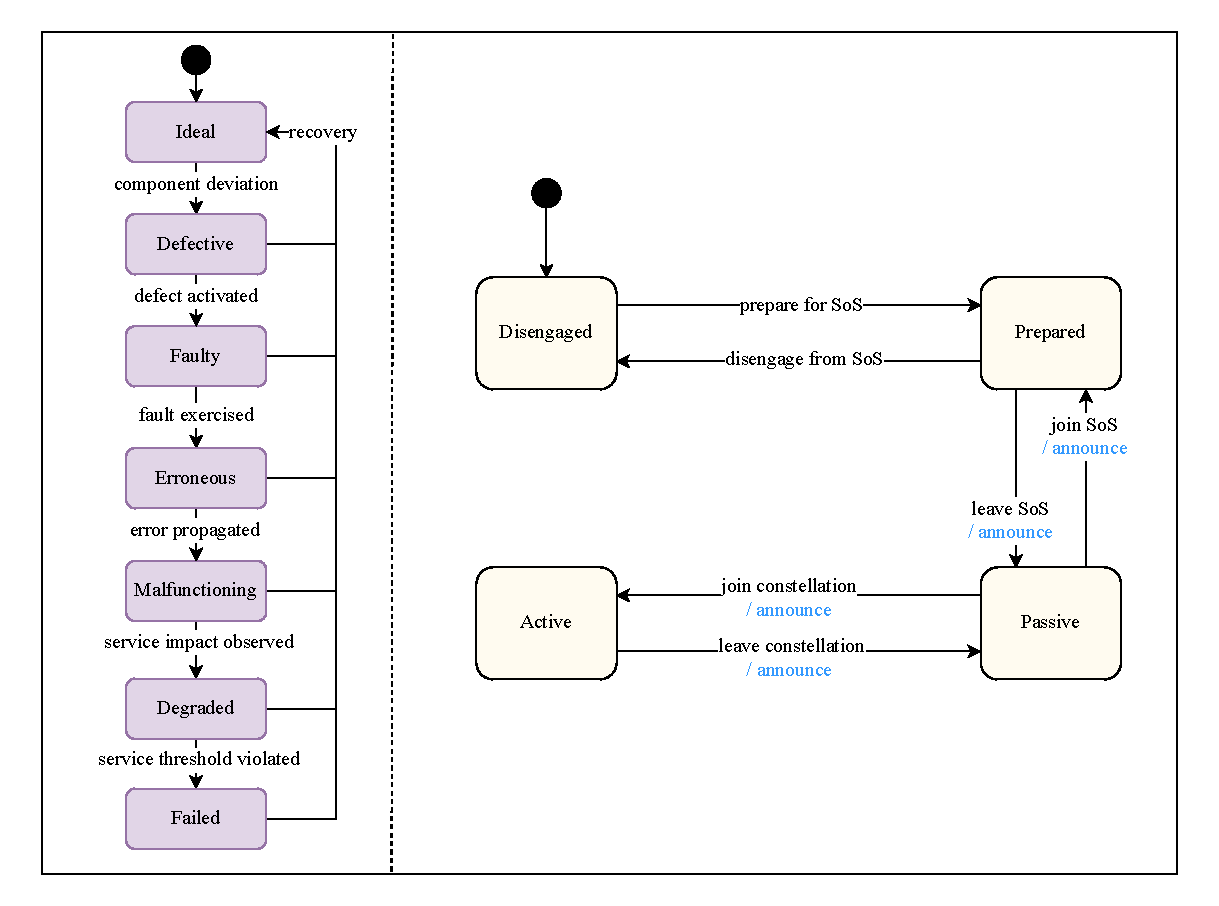
\includegraphics[width=0.65\linewidth]{figures/Approach/lv1.pdf}
\caption{Level 1}
\label{fig:sos-lifecycle-model-lvl-1}
\end{figure}



\subsubsection{Level 2: Proactive}

Level 2 introduces a \textit{Pending} and \textit{Participating} sub-states within the \textit{Active} state to enforce departure notice. While \citet{axelsson2019refined} discusses obligations and cost-benefit considerations, the original lifecycle allows for immediate withdrawal. If dependencies or commitments exist, however, abrupt departure may destabilize ongoing service delivery. The refined state chart inserts a temporal buffer between departure announcement and final exit. During this notice period, the constituent remains operational while other systems adapt their behavior.

This refinement directly addresses disturbances caused by constituent evolution and temporary inability to meet demand. Participation changes are no longer abrupt. Instead, adaptation can begin before capability loss occurs. Intervention shifts to a point before the disturbance impact, reducing cascading effects.

\begin{figure}[htp]
\centering
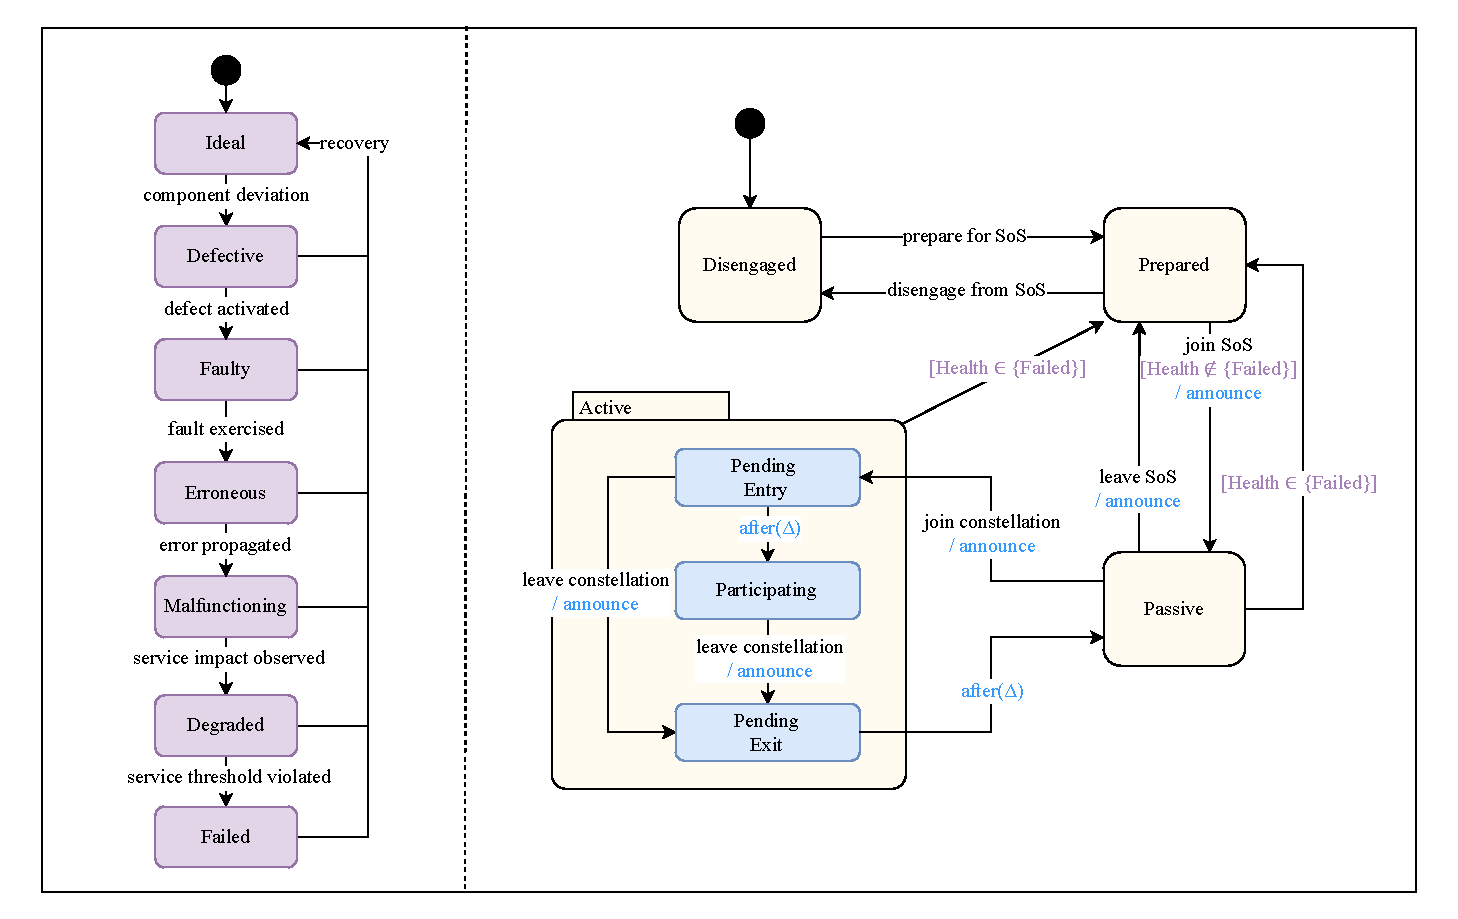
\includegraphics[width=0.65\linewidth]{figures/Approach/lv2.pdf}
\caption{Level 2}
\label{fig:sos-lifecycle-model-lvl-2}
\end{figure}




\subsubsection{Level 3: Controlled}
Level 3 formalizes negotiation and obligation enforcement within the lifecycle. \citet{axelsson2019refined} explicitly references contractual and monetary arrangements during joining and leaving, including compensation models and credential revocation. These imply that participation may be conditional and governed by enforceable commitments.

The refined state chart introduces \textit{Available} and \textit{Negotiating} sub-states prior to admission, enabling constituents to signal readiness before entering formal negotiation. Membership approval becomes conditional, and exit transitions are guarded such that departure is denied while obligations remain active. Membership may also be revoked under defined conditions.

This level mitigates disturbances associated with unstable participation and uncontrolled constituent evolution. Unsafe or non-compliant systems may be denied entry, and obligated participants cannot withdraw in ways that jeopardize capability delivery. Intervention now occurs before structural integration or withdrawal, preventing disturbance formation rather than compensating for its consequences.


\begin{figure}[htp]
\centering
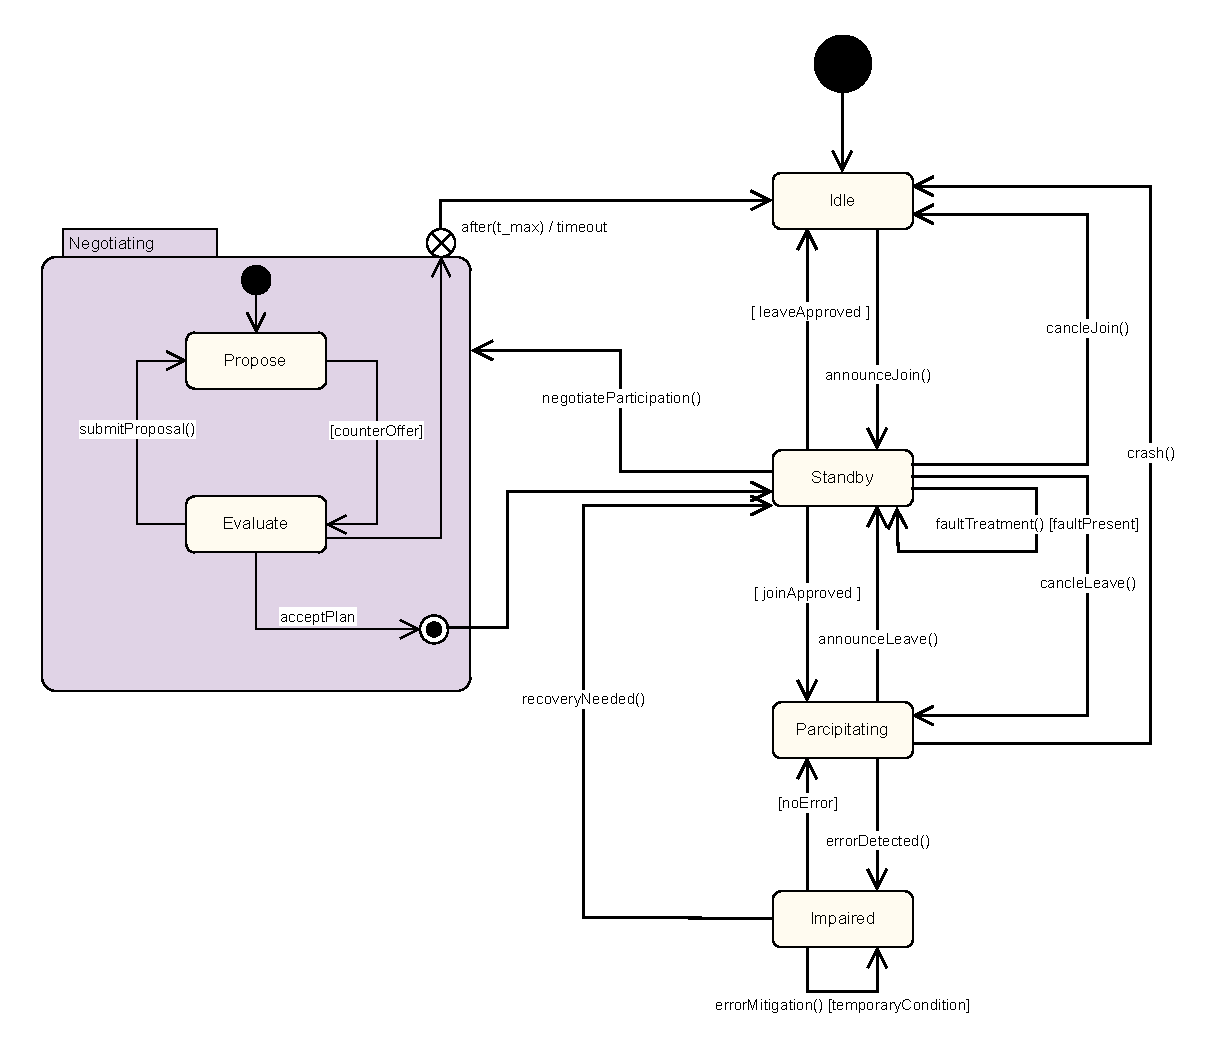
\includegraphics[width=0.85\linewidth]{figures/Approach/lv3.pdf}
\caption{Level 3}
\label{fig:sos-lifecycle-model-lvl-3}
\end{figure}




\subsubsection{Level 4: Adaptive}

\citet{axelsson2019refined} describes how constituents join constellations to deliver capabilities but does not explicitly model how the SoS adapts when a constituent leaves and capability delivery is affected. SoS research emphasizes dynamic reconfiguration to compensate for structural loss, including architectural reallocation, role reassignment, and runtime composition under disruption (\cite{fang2020improving, fang2024integrated, manzano2020dynamic, pradhan2016achieving, pape2013fuzzy, petitdemange2016assisting, mohsin2019modeling, derhamy2019system, blair2015holons}).

Level 4 integrates this principle directly into the lifecycle by refining the \textit{Participating} state into \textit{Performing Role} and \textit{Adjusting Role} sub-states. The SoTS may enforce role reassignment to preserve capability, while constituents may formally request role changes or withdraw if reassignment is unacceptable.

The state chart now controls both participation and functional allocation. This level directly addresses disturbances arising from interdependencies and undesired emergent behavior by enabling structural reconfiguration before capability breakdown occurs.  The SoTS adapts its composition and role distribution to preserve mission delivery and prevents the pre conditions for the disturbance from arising.


\begin{figure}[htp]
\centering
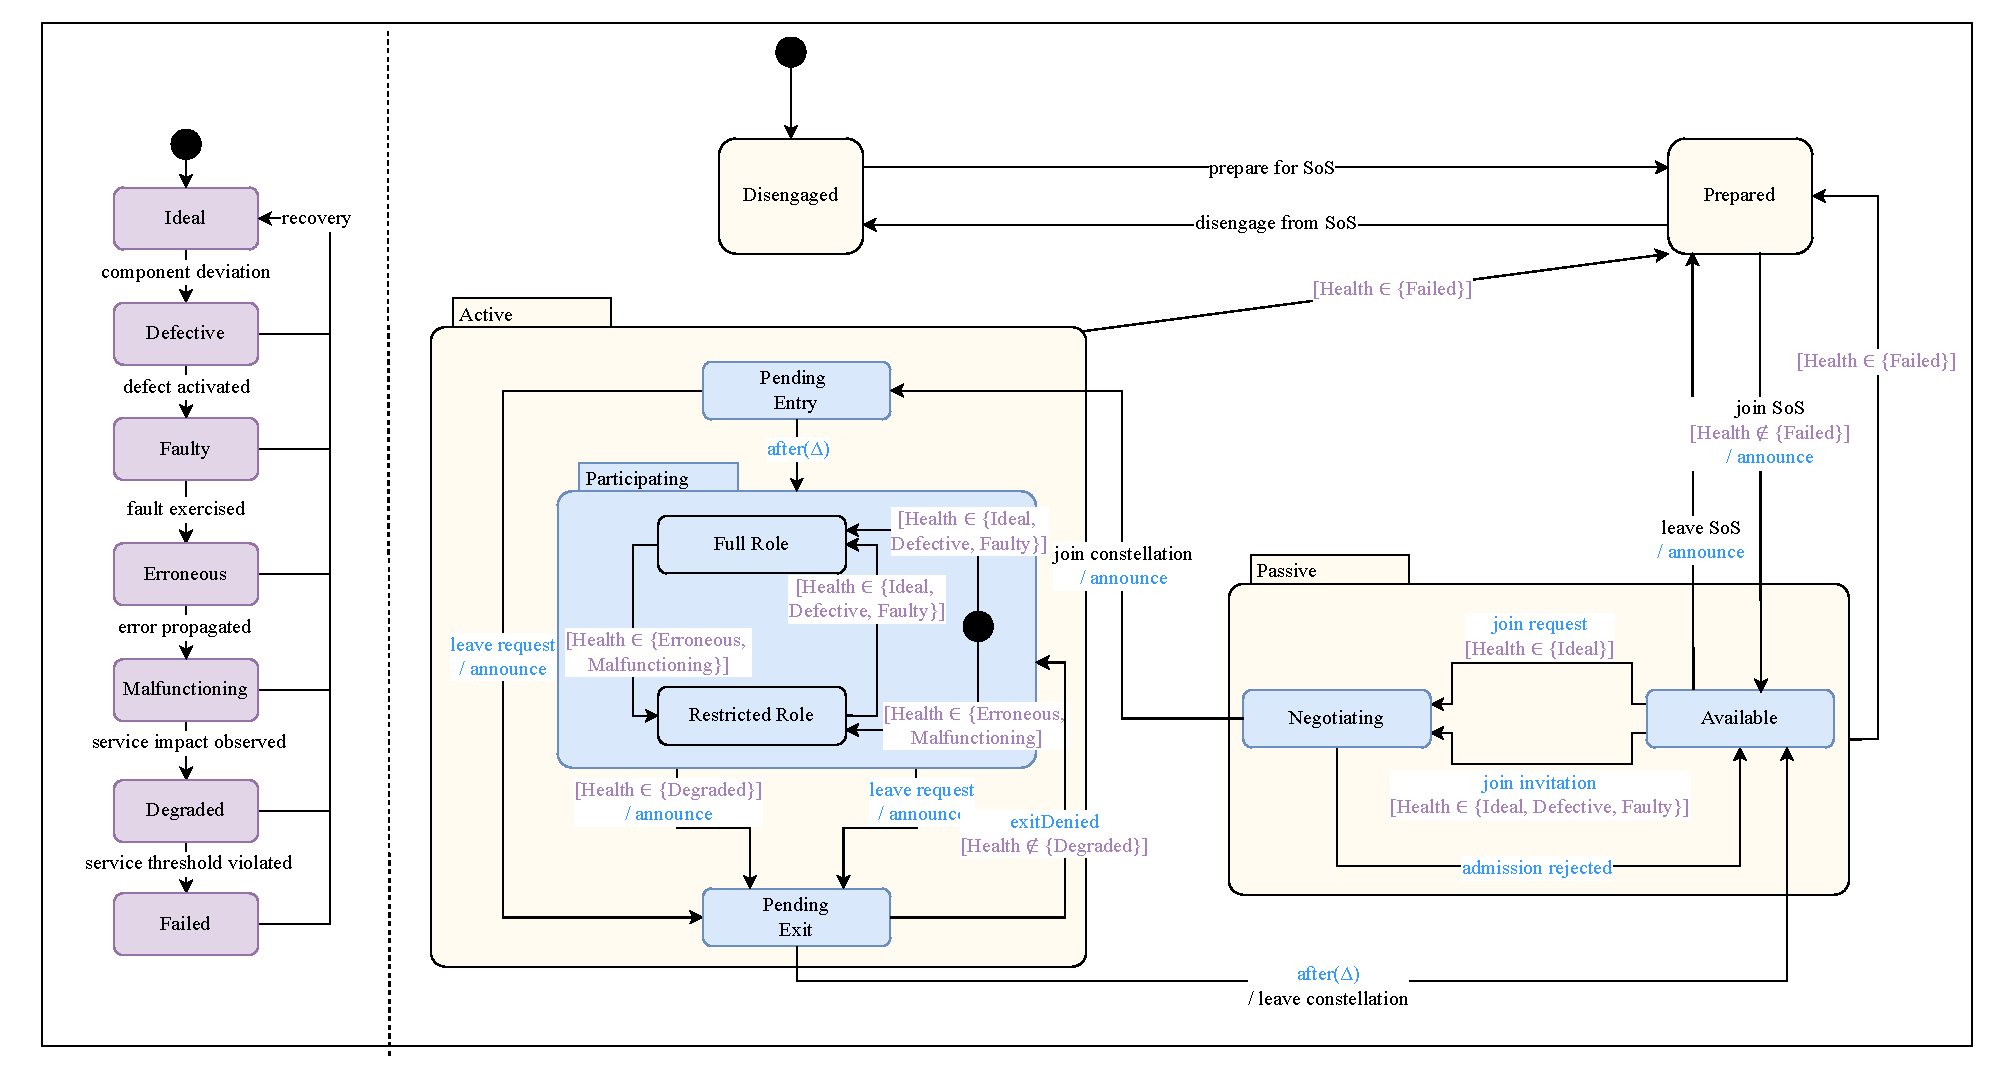
\includegraphics[width=0.85\linewidth]{figures/Approach/lv4.pdf}
\caption{Level 4}
\label{fig:sos-lifecycle-model-lvl-4}
\end{figure}





\subsection{Compatibility with SoTS Types}
\begin{table}[htp]
\centering
\footnotesize
\begin{tabular}{p{1.7cm} c c c c c c}
\toprule
\textbf{Reliability Level} 
& \textbf{Directed} 
& \textbf{Acknowledged} 
& \textbf{Collaborative} 
& \textbf{Virtual} 
& \textbf{Spec. DT}
& \textbf{Spec. DT + PT} \\
\midrule

Reactive     & X & X & X & X & X & X \\
Proactive    & X & X & X &   & X & X \\
Controlled   & X & X &   &   & X & X \\
Adaptive     & X &   &   &   & X & X \\

\bottomrule
\end{tabular}
\caption{Compatibility of reliability levels with SoTS types}
\end{table}
The feasibility of implementing the levels of reliability depends on the coordination authority and managerial independence of the SoTS (\secref{ch:literature-review}). Directed SoTS, and specialized DT-based systems, support higher reliability levels due to centralized or structurally embedded control. Acknowledged SoTS can implement controlled participation through negotiation, though full adaptive reconfiguration may be limited by constituent autonomy. Collaborative and virtual SoTS prioritize independence and emergent coordination, constraining the applicability of strong lifecycle regulation. High levels of reliability are not universally applicable. Greater constituent autonomy increases exposure to disturbances and shifts responsibility toward service-level fault tolerance. Stronger coordinating authority enables earlier architectural intervention and reduces reliance on reactive recovery mechanisms.



\subsection{Orthogonal State Machine: Lifecycle and Operational Health Integration}
\citet{parhami2002defect} proposes operational states that reflect the capability of a system over time. As discussed previously, participation in a SoTS is tied to capability; therefore, the operational condition of a constituent also affects its ability to participate.

We extend the previously introduced lifecycle state machines by incorporating an orthogonal parallel region representing constituent health. In this formulation, lifecycle participation and operational reliability are modeled separately but interact through defined transition constraints. Changes in constituent health may therefore enforce or restrict participation decisions within the SoTS.

\textbf{TODO ONCE RELIABILITY STATES ARE FINALIZED AND PREVIOUS STATE MACHINES ARE GIVEN FEEDBACK BY PROF}


INITAL IDEAS
\begin{figure}[htp]
\centering
\includegraphics[width=0.85\linewidth]{figures/Approach/lv1_rel.pdf}
\caption{Level 4}
\label{fig:sos-lifecycle-model-lvl-1-o}
\end{figure}


\begin{figure}[htp]
\centering
\includegraphics[width=0.85\linewidth]{figures/Approach/lv2_rel.pdf}
\caption{Level 4}
\label{fig:sos-lifecycle-model-lvl-2-o}
\end{figure}



\begin{figure}[htp]
\centering
\includegraphics[width=0.85\linewidth]{figures/Approach/lv3_rel.pdf}
\caption{Level 4}
\label{fig:sos-lifecycle-model-lvl-3-o}
\end{figure}



\begin{figure}[htp]
\centering
\includegraphics[width=0.85\linewidth]{figures/Approach/lv4_rel.pdf}
\caption{Level 4}
\label{fig:sos-lifecycle-model-lvl-4-o}
\end{figure}



